Med informationerne fra domænemodellen er der udviklet en række diagrammer ud fra applikationsmodellen.
Applikationsmodellen er en metode til at fin-tænke software designet inden man går i gang med implementeringen. Ud fra de aktuelle Usecases er funktionaliteten beskrevet med sekvensdiagrammer i figur \ref{fig:PC_SD1} og figur \ref{fig:PC_SD2}.

\begin{figure}[H] \centering
     {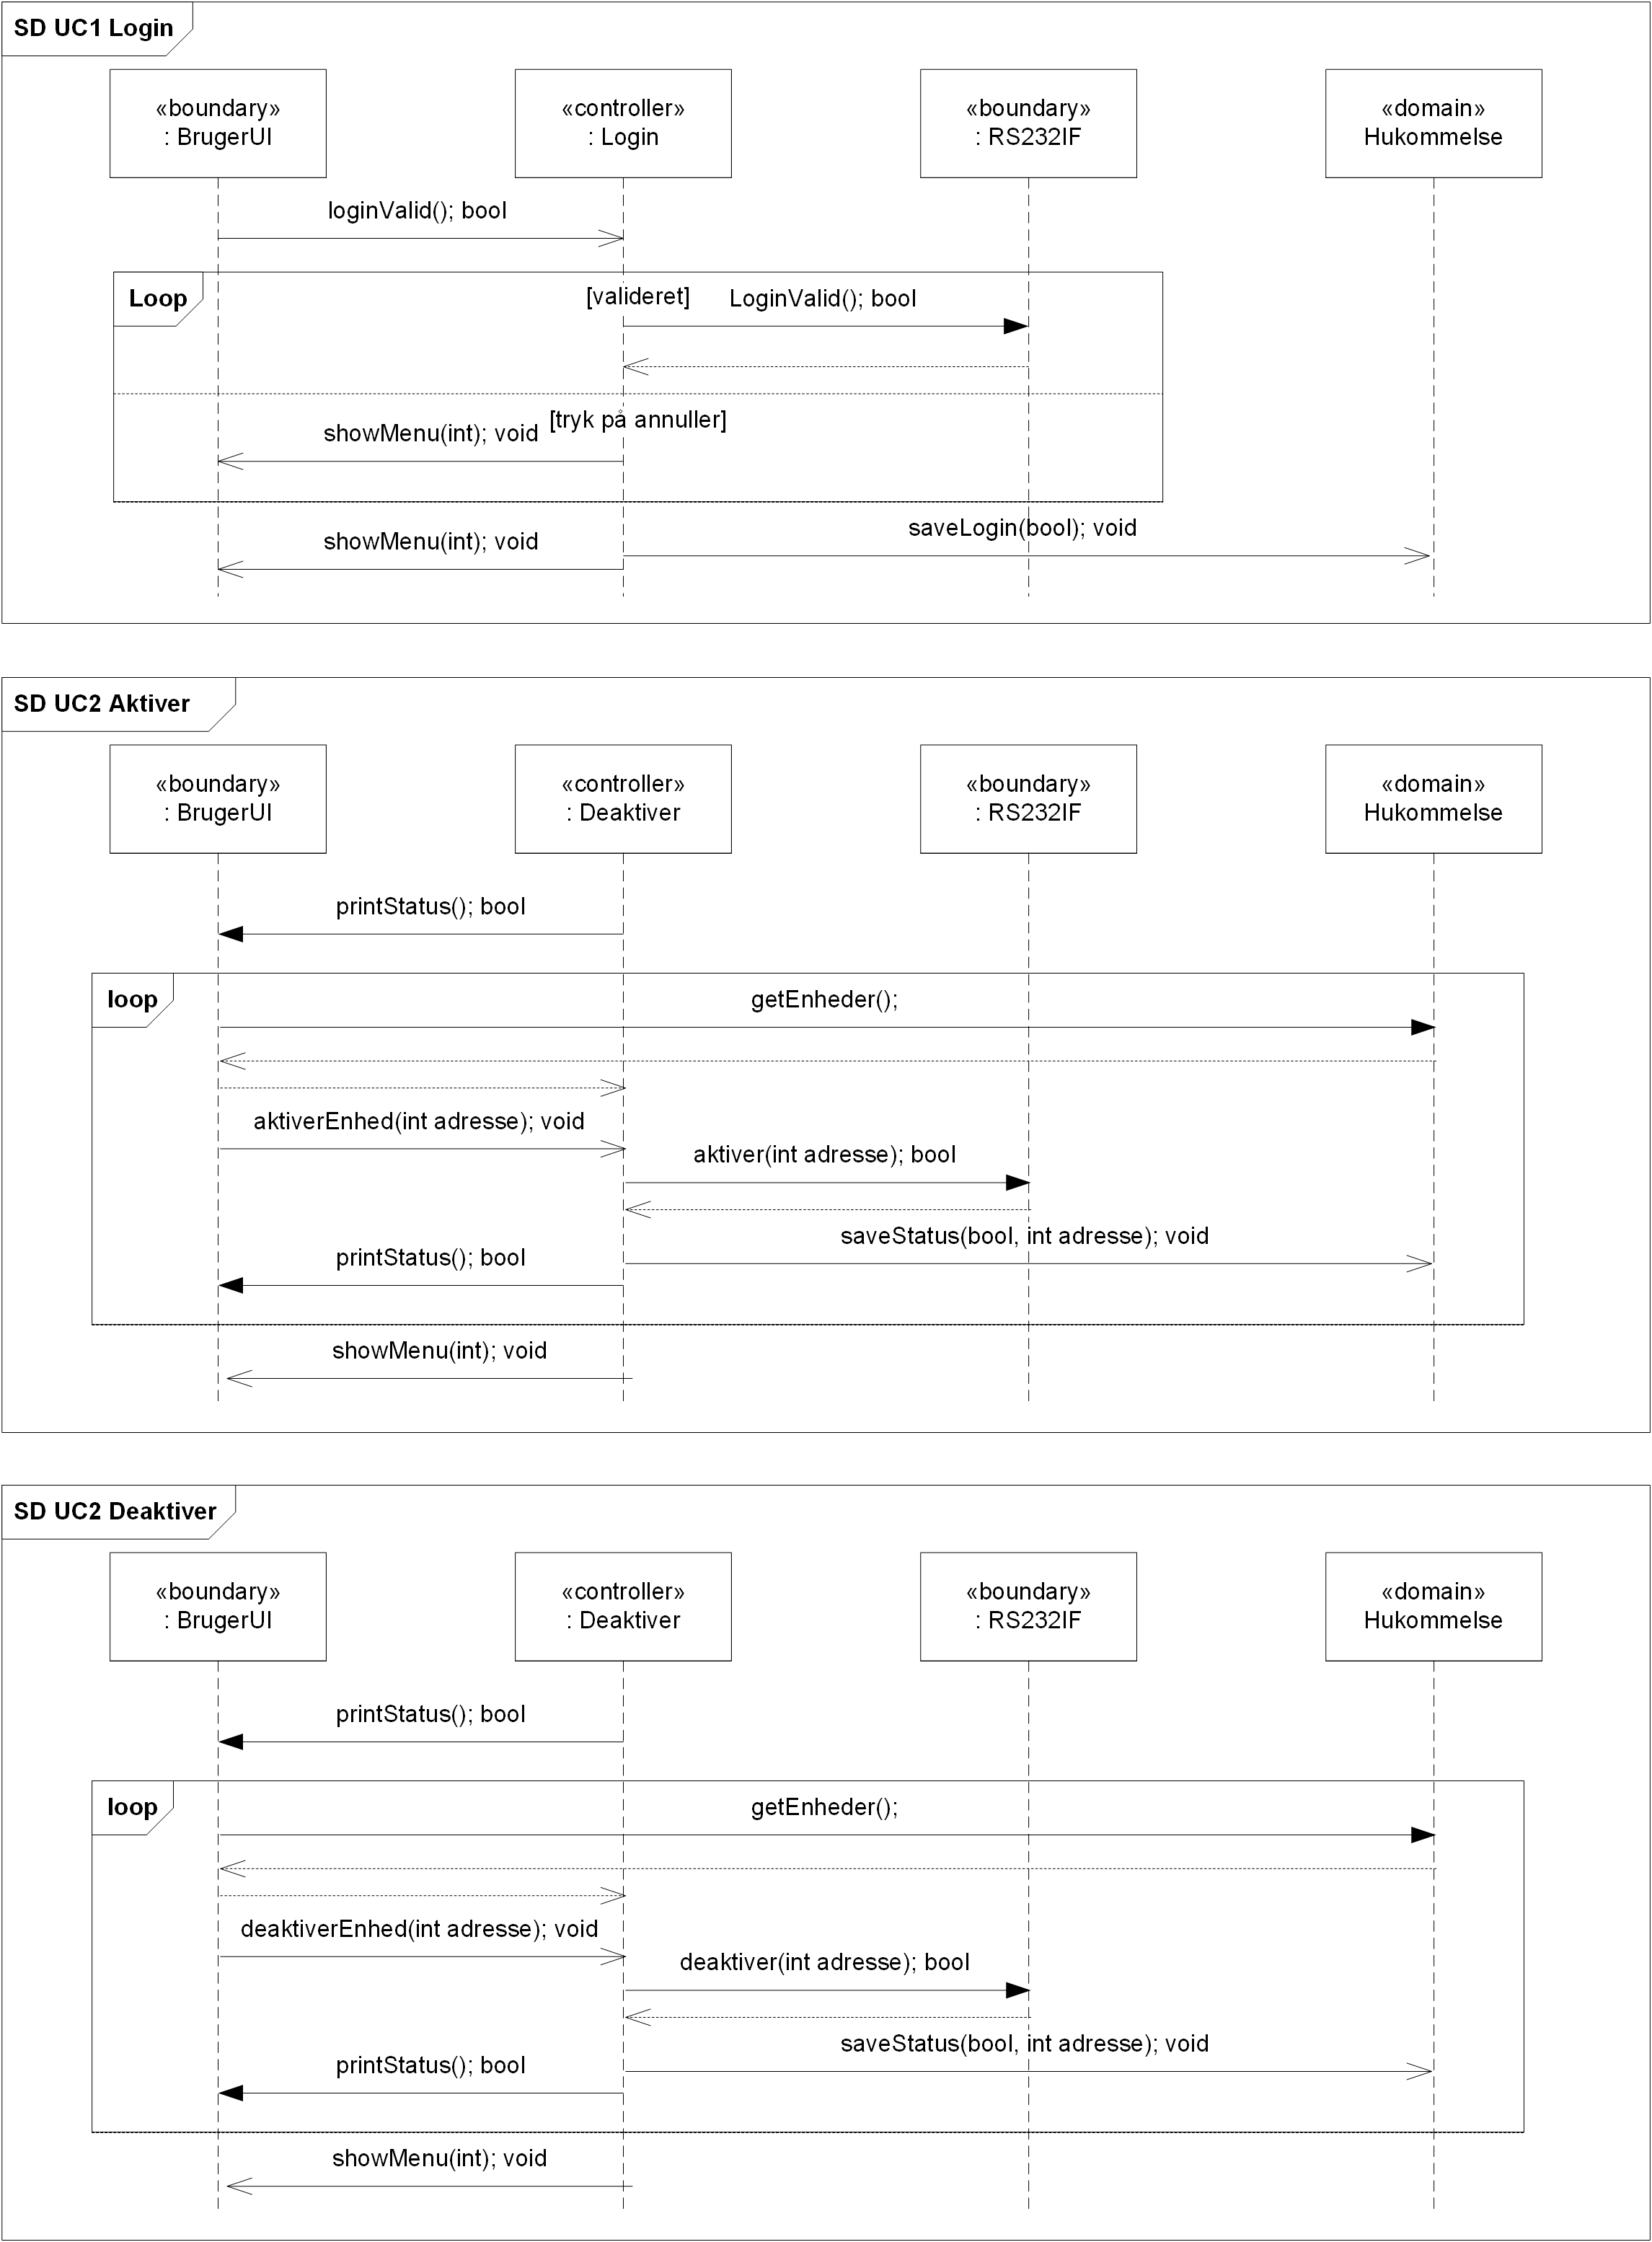
\includegraphics[width=0.9\textwidth]{billeder/uml/PC_SD1}}
     \caption{Use-case 1-3 sekvensdiagram for PC}
     \label{fig:PC_SD1}
\end{figure}
\clearpage

\begin{figure}[H] \centering
     {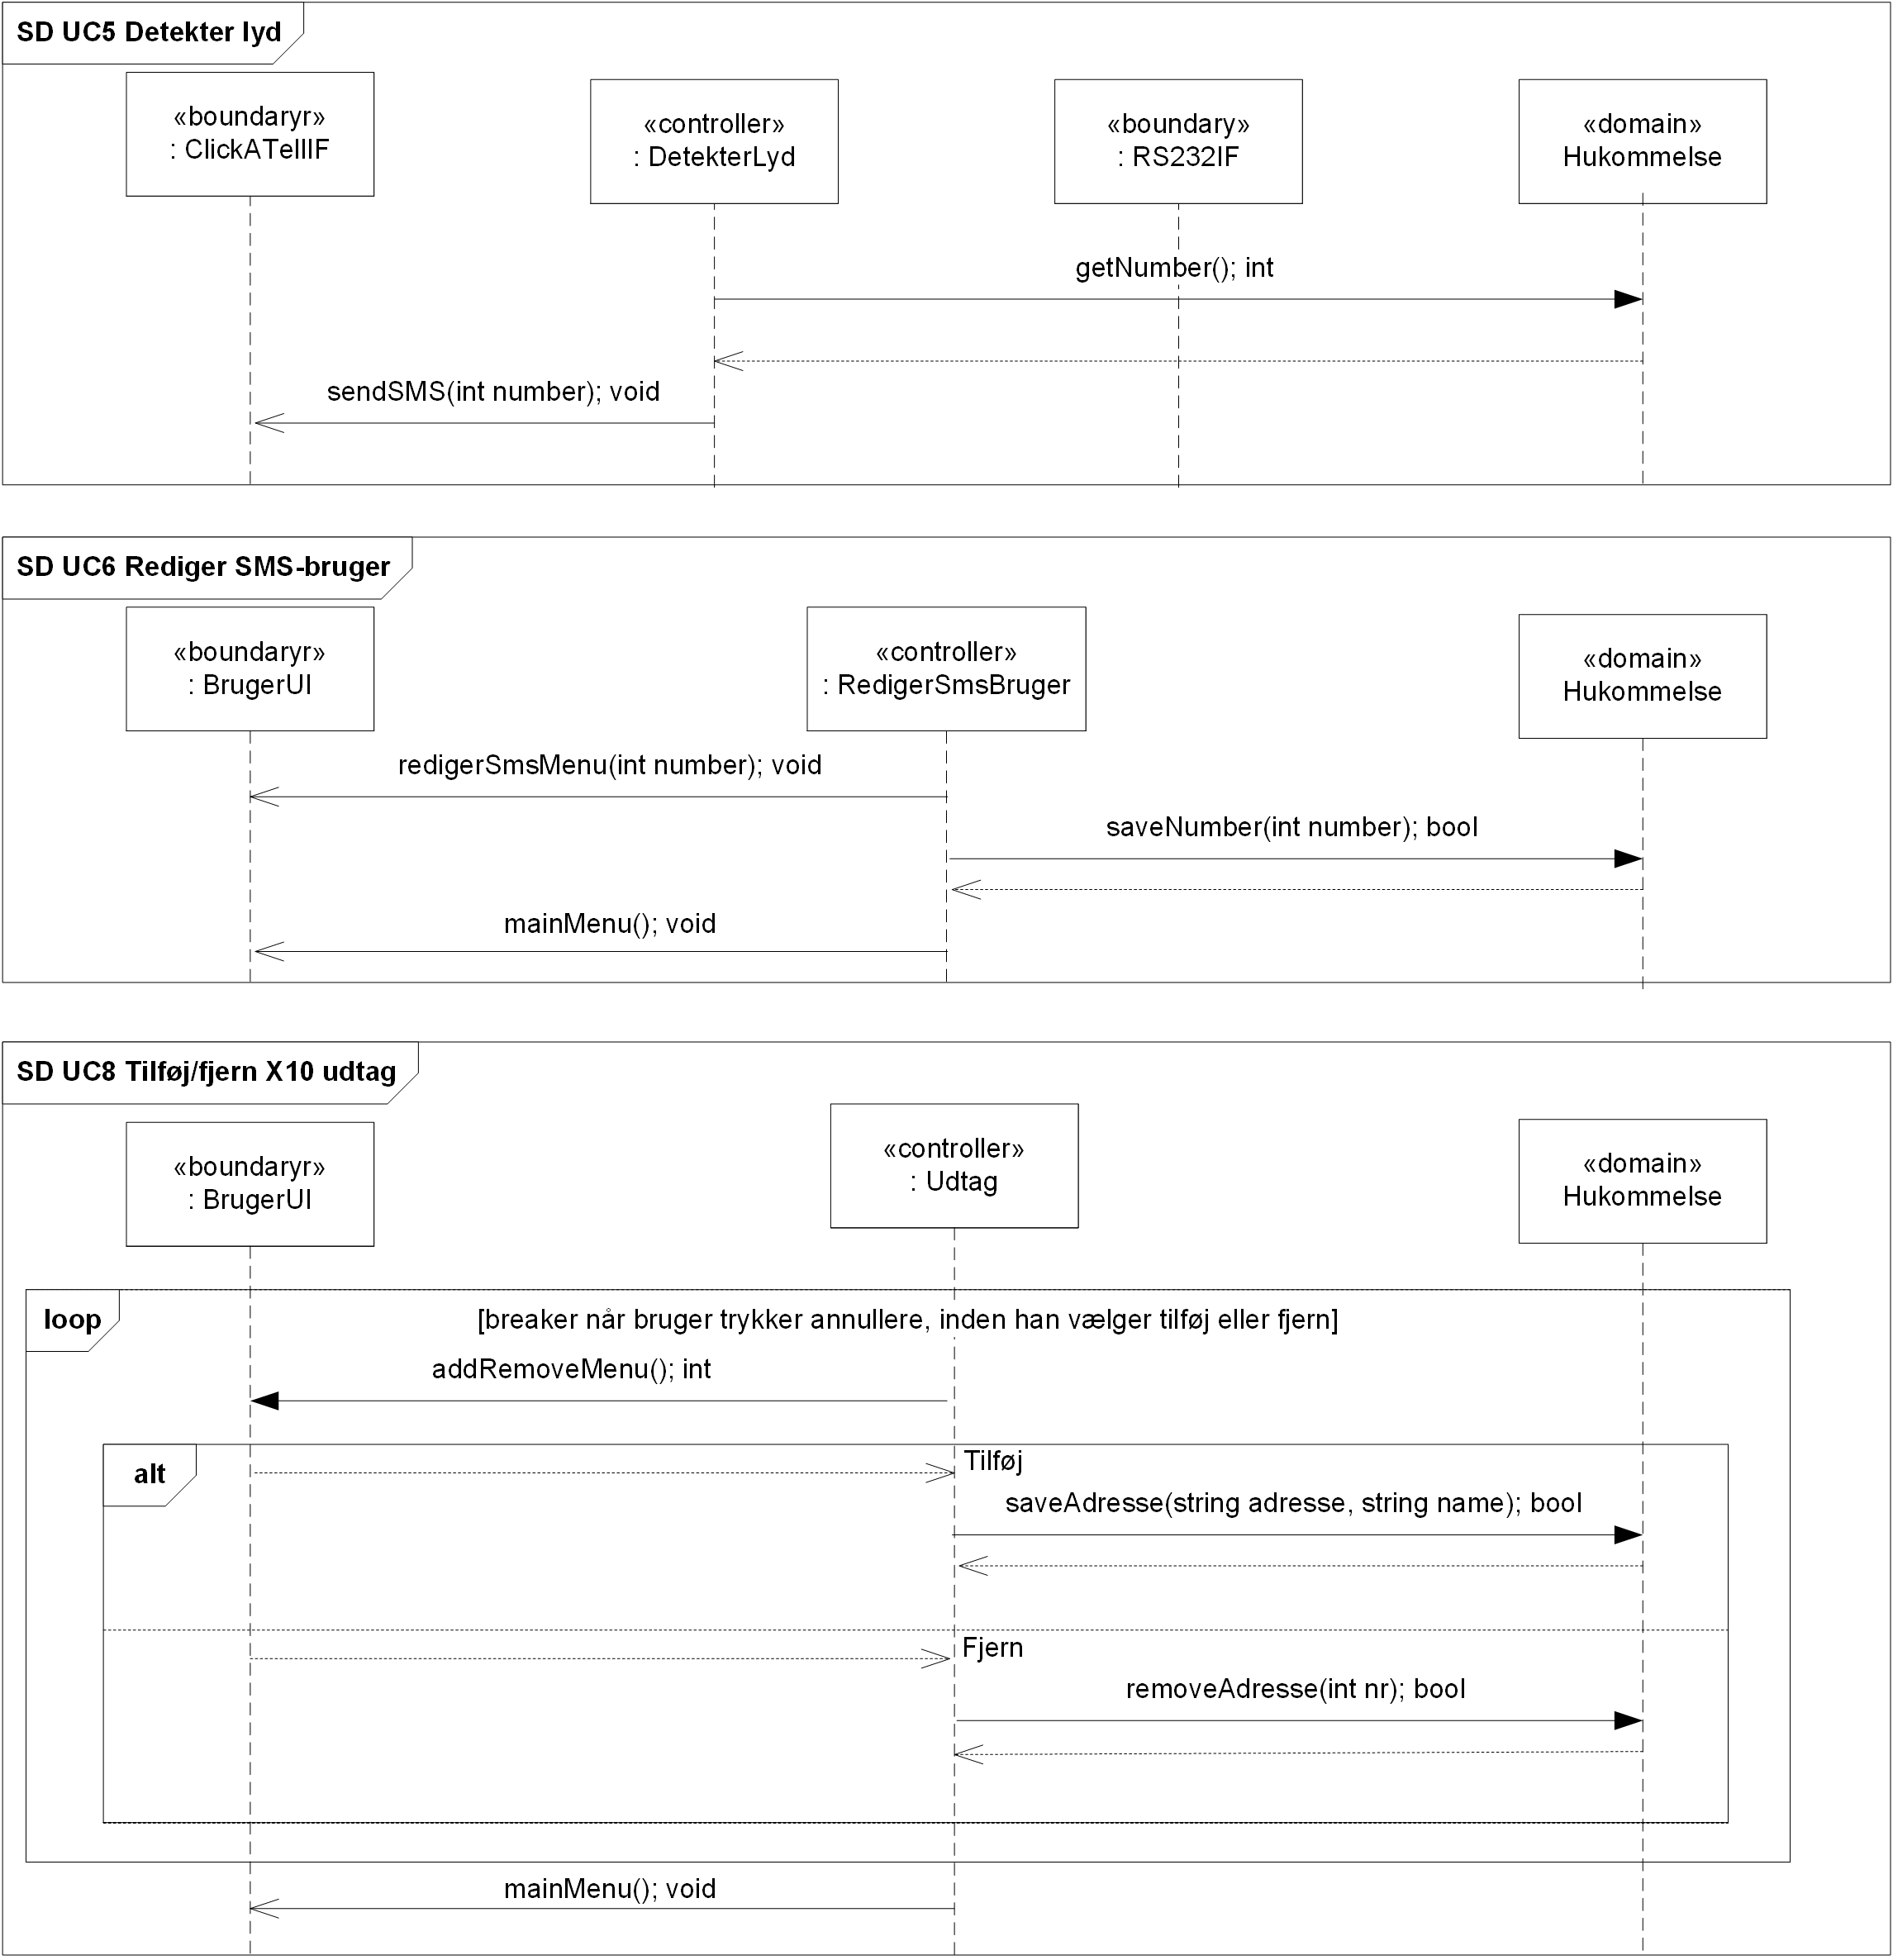
\includegraphics[width=0.9\textwidth]{billeder/uml/PC_SD2}}
     \caption{Use-case 5-8 sekvensdiagram for PC}
     \label{fig:PC_SD2}
\end{figure}

\clearpage

Alle kaldene til controller-klasserne kommer fra main.cpp programmet som tager imod brugerinputs i preLogin menuen og mainMenuen. Når mainMenuen er vist så står main.cpp og spørger på read() metoden i RS232IF klassen som tester om den har modtaget data fra STK500-kittet. Dette gør den for at se om login status har ændret sig eller om der skal sendes en sms til brugeren pga. babyalarmen.\\
Metode navnene i controller-klasserne kan ses på næste sidste i klassediagrammet som er lavet på baggrund af Sekvens-diagrammerne.

\begin{figure}[H]
     {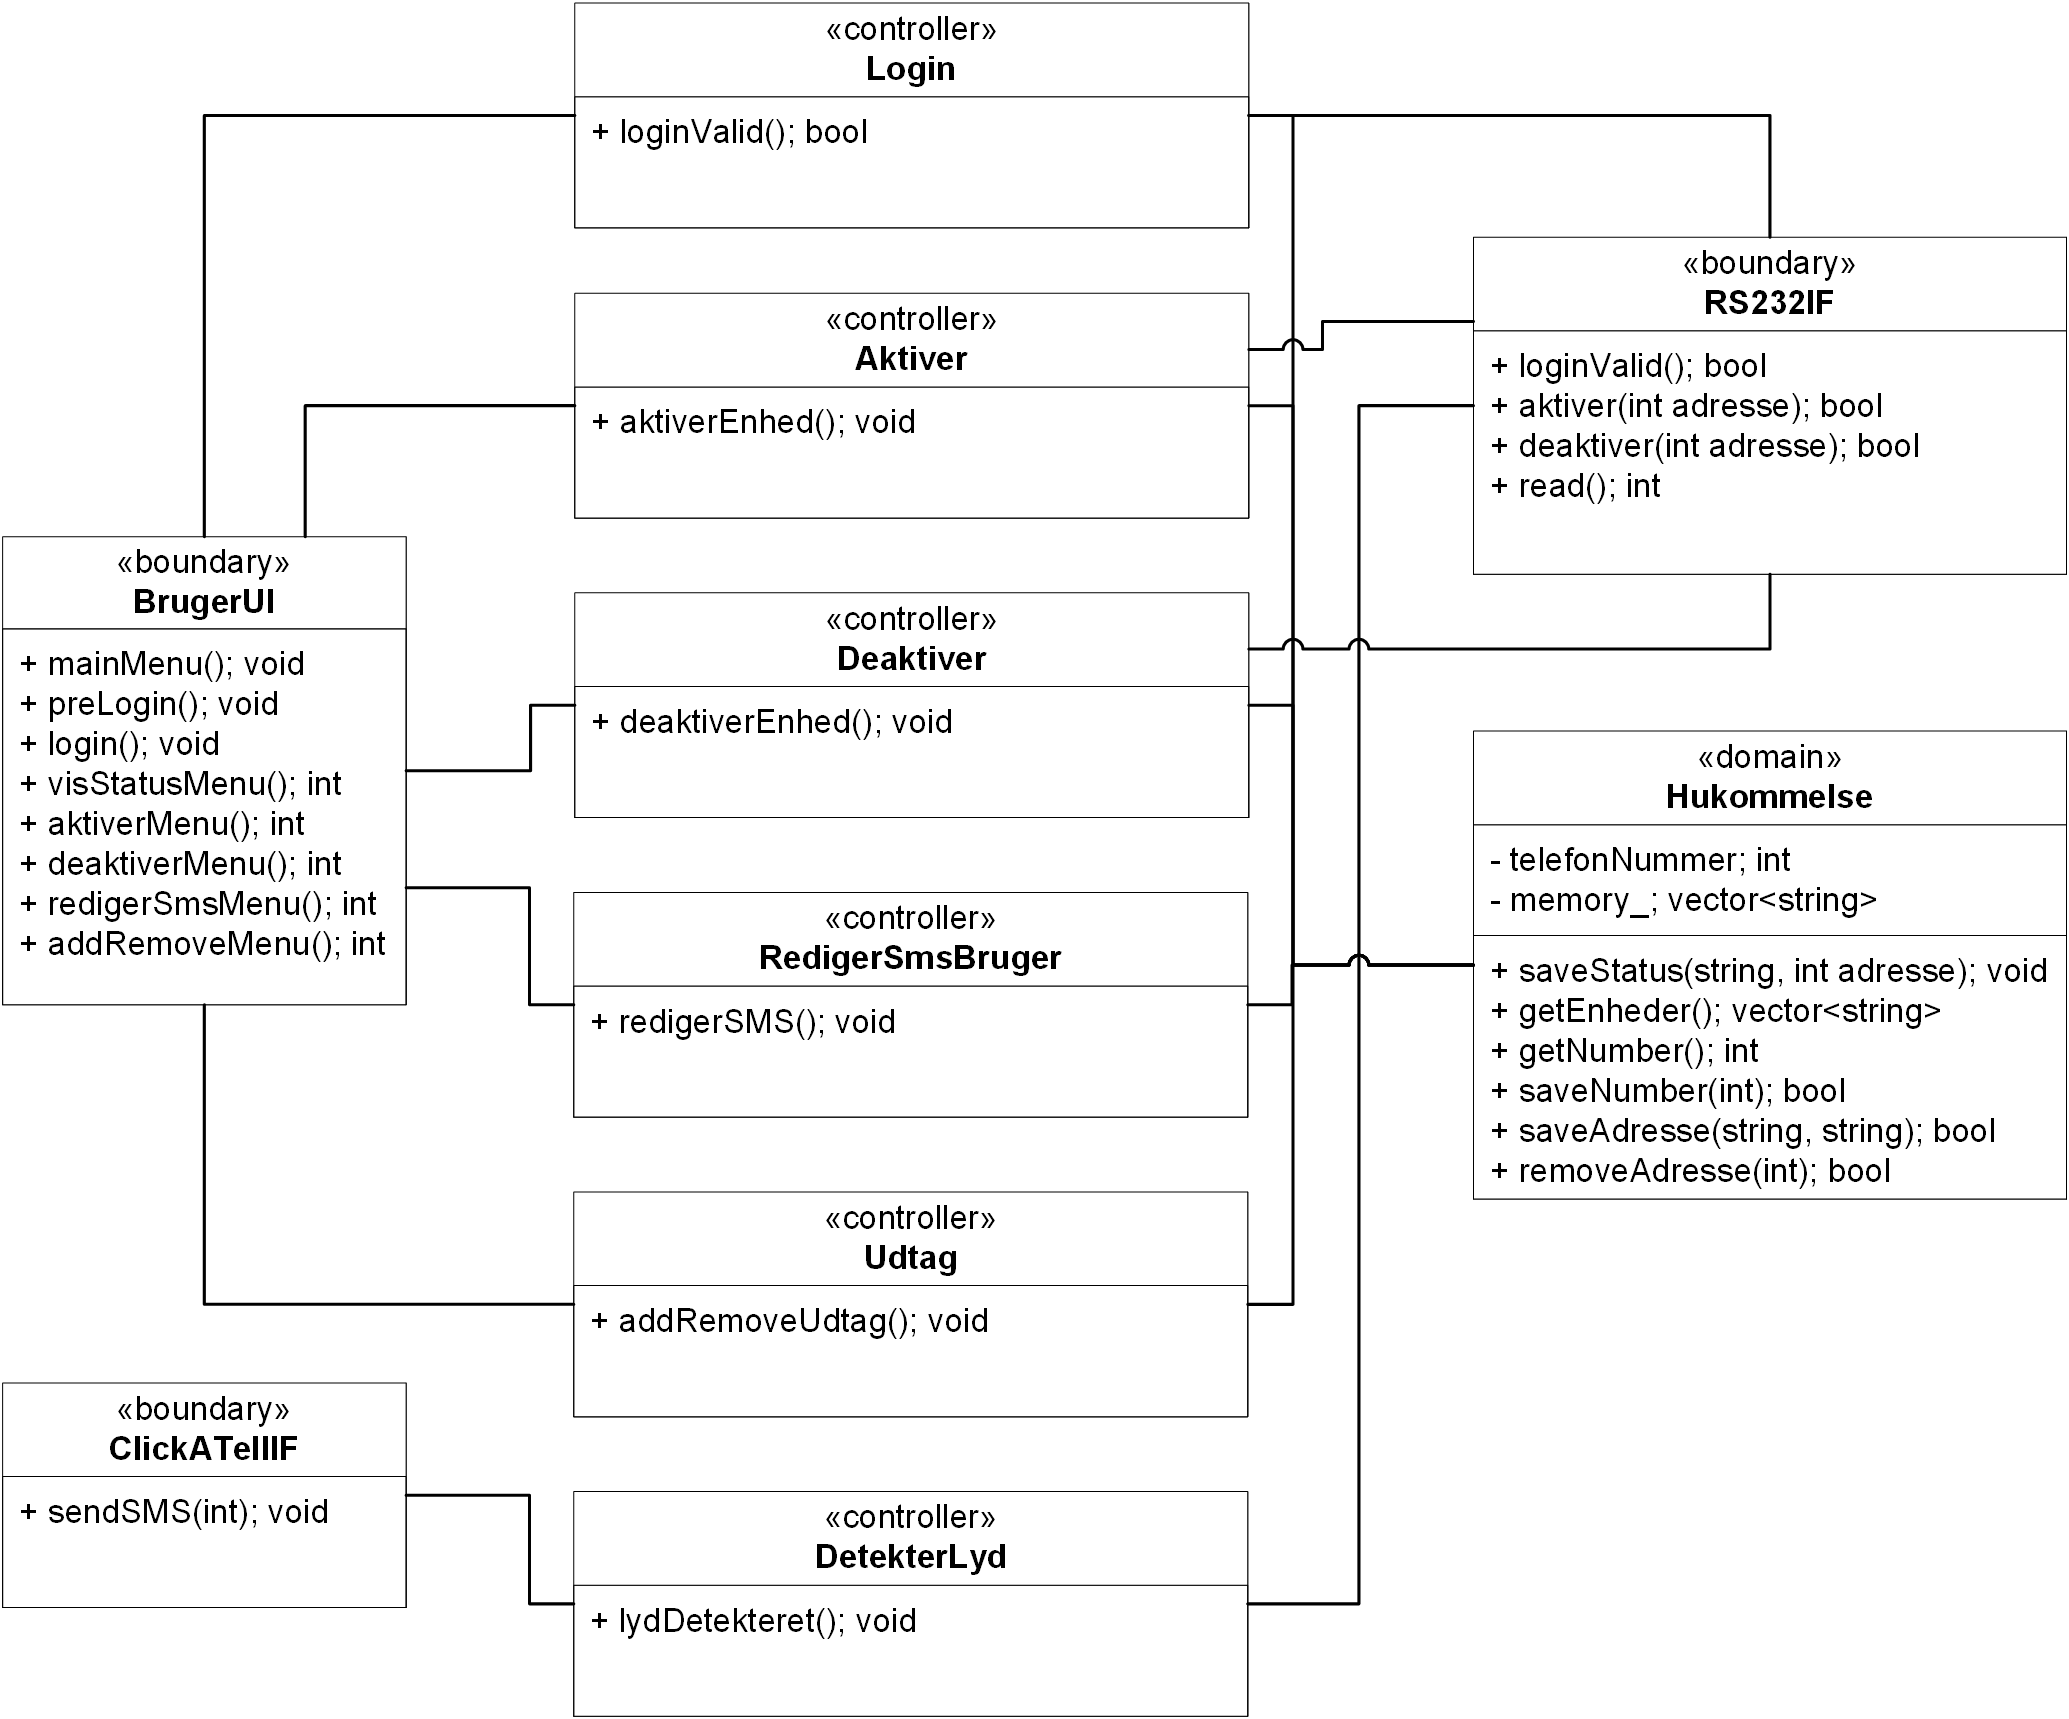
\includegraphics[width=\textwidth]{billeder/uml/PC_Class}}
     \caption{Klassediagram for PC}
     \label{fig:PC_Class}
\end{figure}

\clearpage
\vspace*{30 px}
\begin{figure}[H]
     {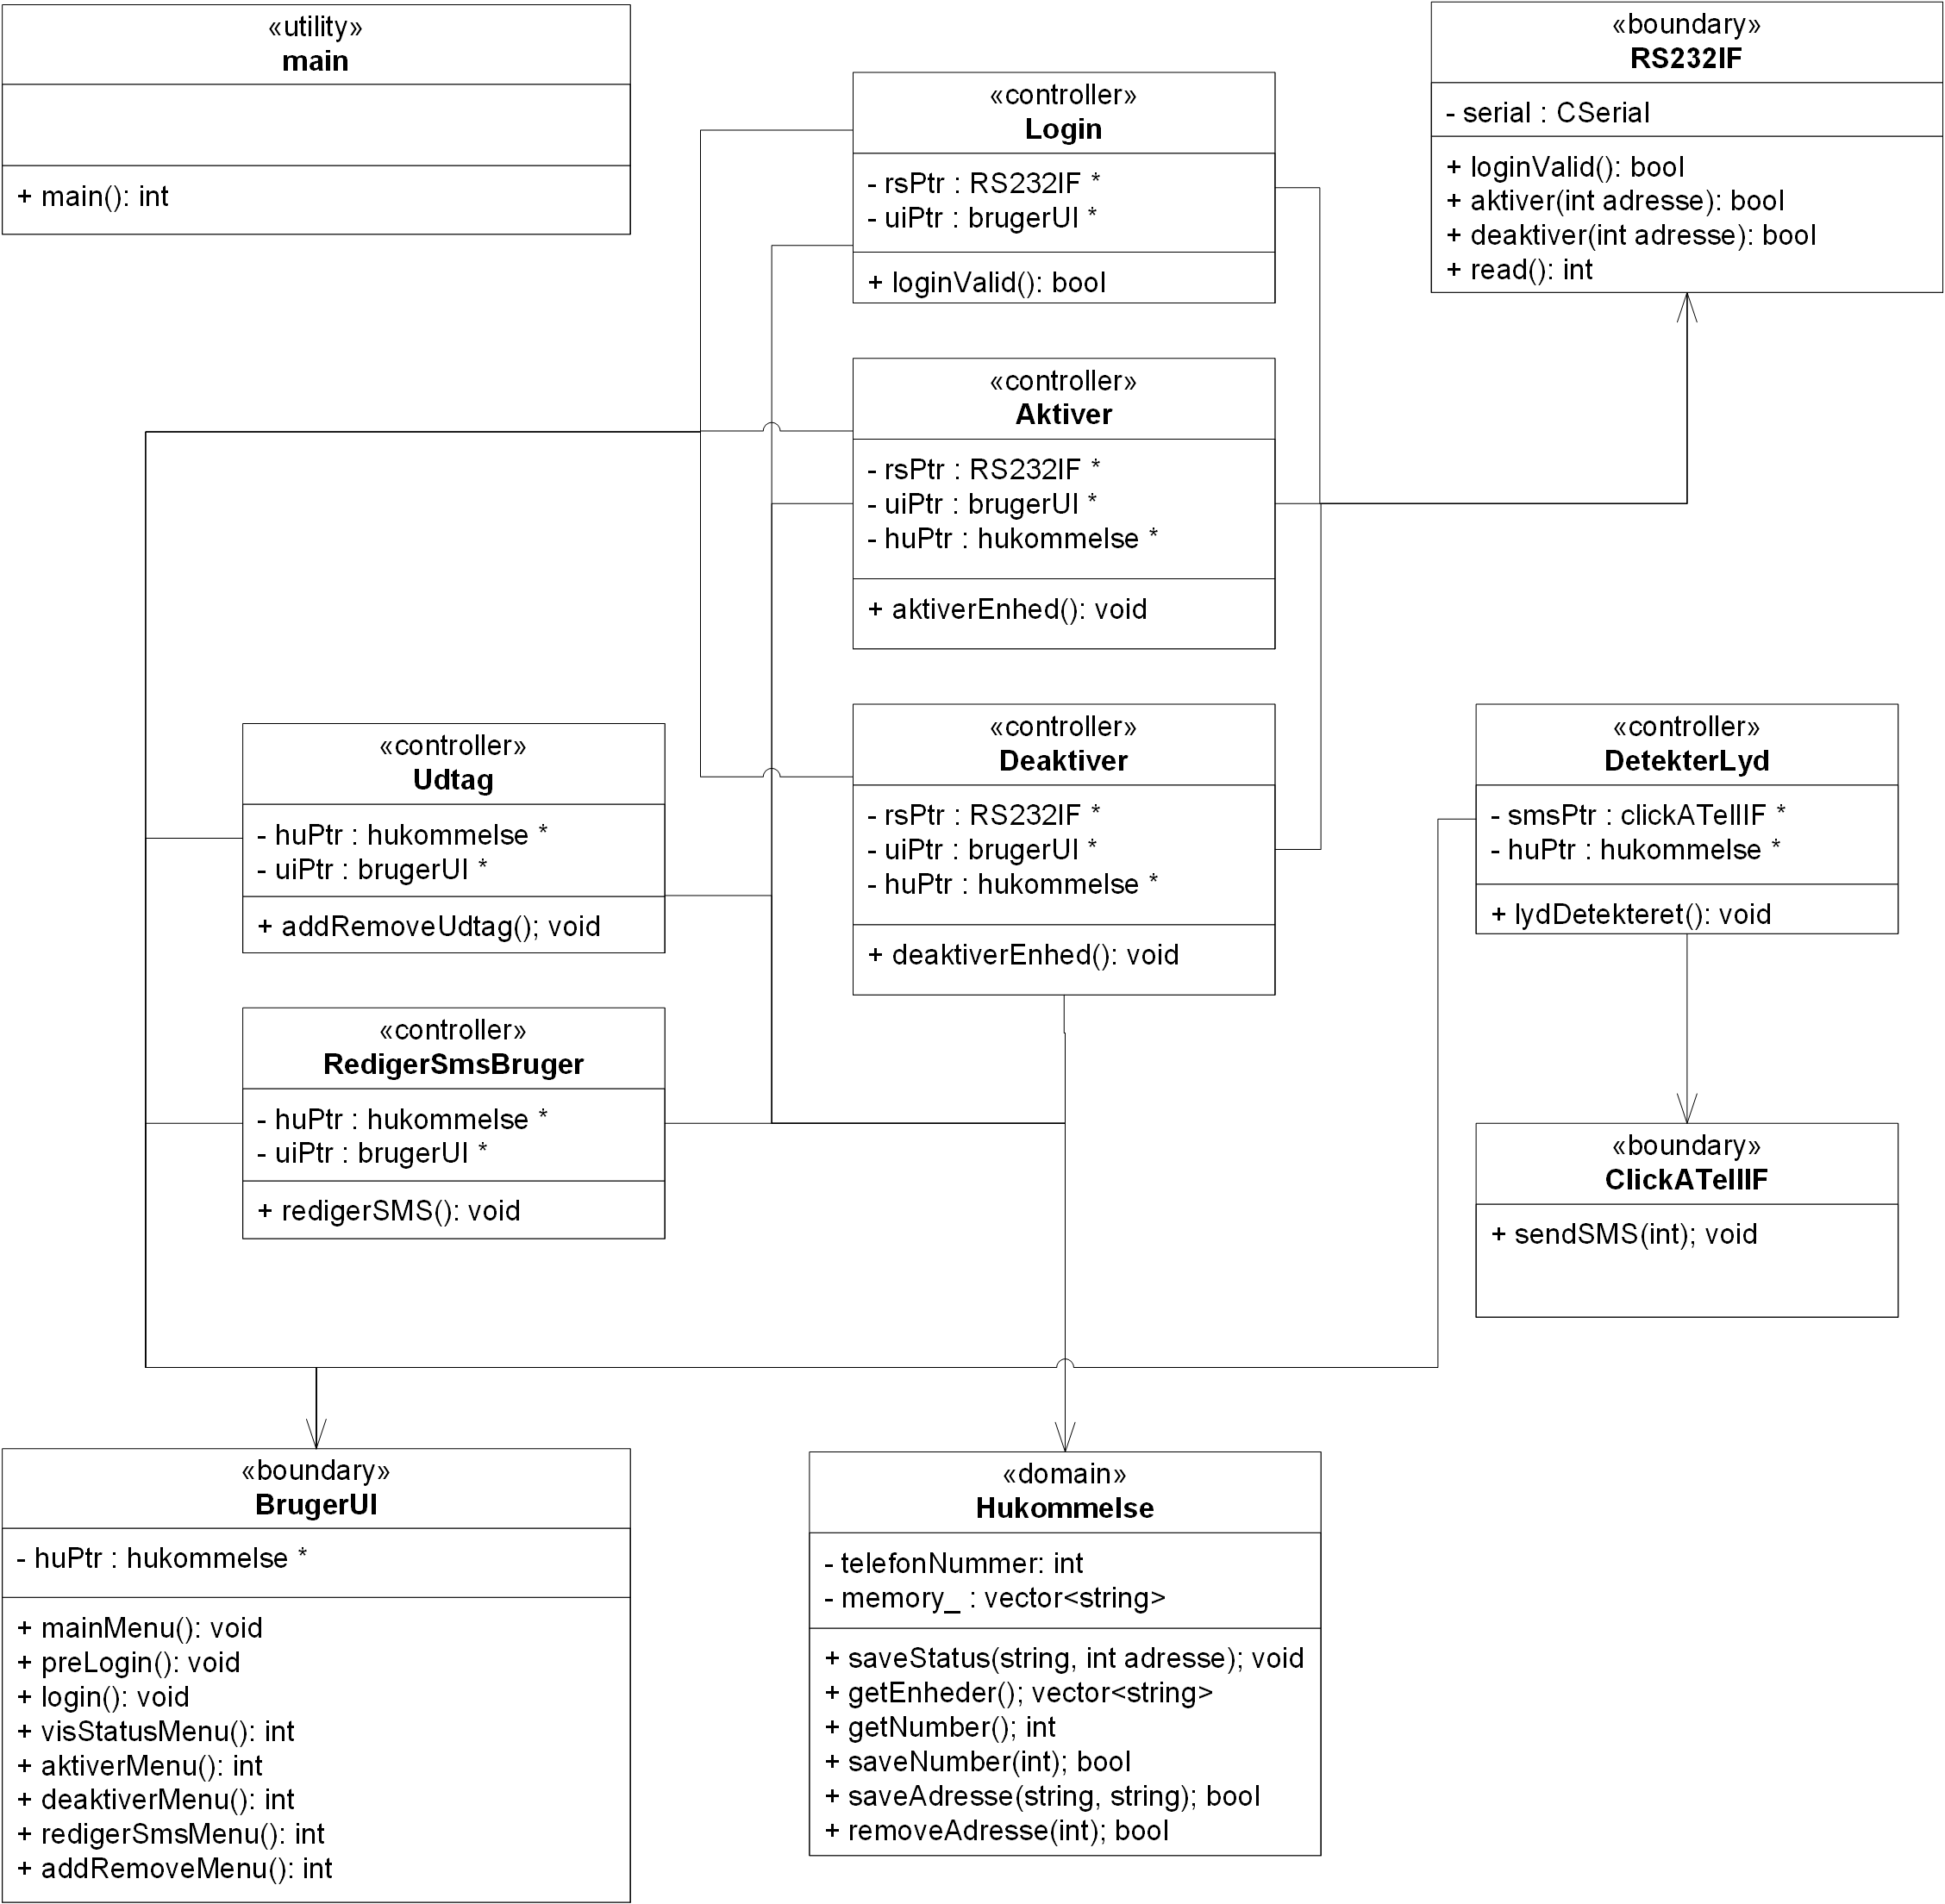
\includegraphics[width=\textwidth]{billeder/uml/PC_Class_static}}
     \caption{Statisk klassediagram for PC}
     \label{fig:PC_Class_Static}
\end{figure}

Main opretter alle objekterne og pointerne til de klasser hvis constructor skal bruge dem. Derudover styre main hvilke controllers der bliver kaldt alt efter bruger input. RS232IF benytter sig at et CSerial\footnote{CSerial klassen findes på http://tinyurl.com/mvzmcep. Kildekode og URL genvej findes på CD'en i Reference mappen. Tom Archer and Rick Leinecker, år 1999. [2014-05-27] } objekt som er en klasse der har de 5 mest basale metoder til at sende og læse på en seriel port.
%
%\begin{figure}[!htb]
%     \xput[0.471]{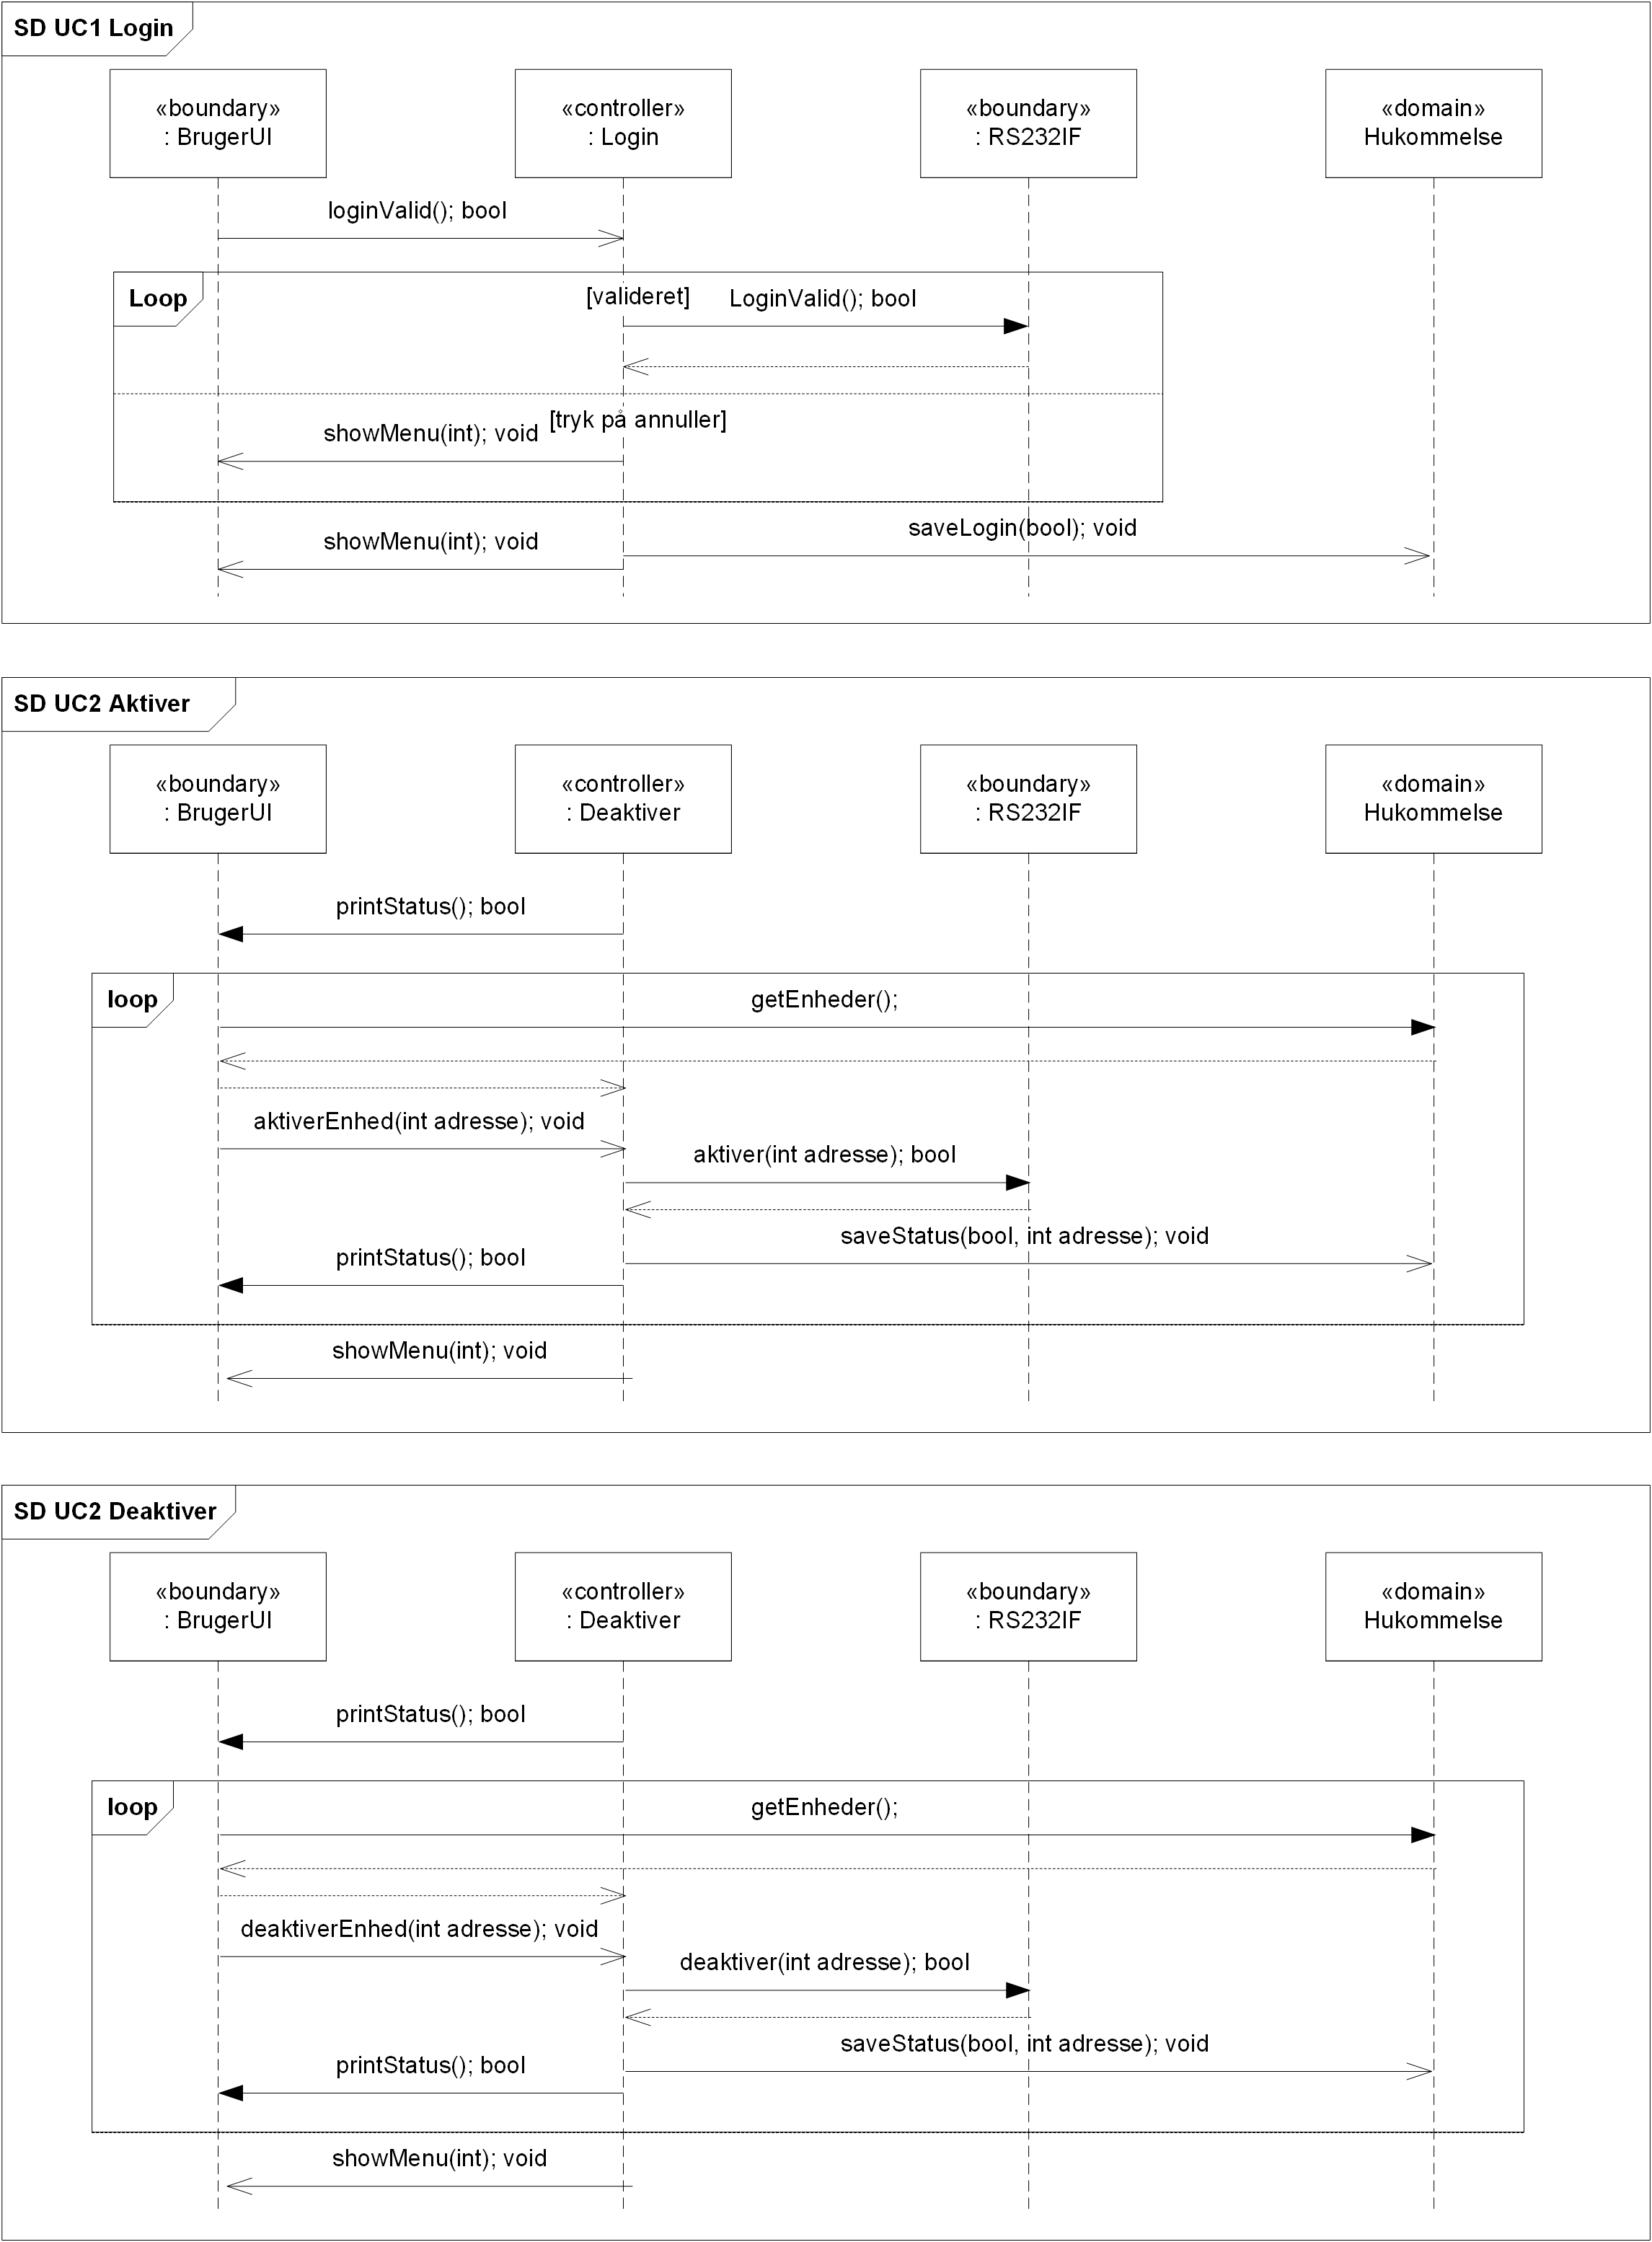
\includegraphics[width=1.32\linewidth]{billeder/uml/PC_SD1}}
%     \caption{Use-case 1-3 sekvensdiagram for PC}
%     \label{fig:PC_SD1}
%\end{figure}
